% Filename: lista1.tex
% 
% This code is part of 'Solutions for MS650, Métodos de Matemática Aplicada II, and F620, Métodos Matemáticos da F\'{i}sica II'
% 
% Description: This file corresponds to the solutions of homework sheet 1.
% 
% Created: 14.07.12 11:13:03 AM
% Last Change: 19.07.12 08:36:46 AM
% 
% Authors:
% - Raniere Silva (2012): initial version
% 
% Copyright (c) 2012 Raniere Silva <r.gaia.cs@gmail.com>
% 
% This work is licensed under the Creative Commons Attribution-ShareAlike 3.0 Unported License. To view a copy of this license, visit http://creativecommons.org/licenses/by-sa/3.0/ or send a letter to Creative Commons, 444 Castro Street, Suite 900, Mountain View, California, 94041, USA.
%
% This work is distributed in the hope that it will be useful, but WITHOUT ANY WARRANTY; without even the implied warranty of MERCHANTABILITY or FITNESS FOR A PARTICULAR PURPOSE.
%
\documentclass[a4paper,12pt, leqno, answers]{exam}
% Filename: paper_size.tex
%
% This code is part of 'Solutions for MS650, Métodos de Matemática Aplicada II, and F620, Métodos Matemáticos da F\'{i}sica II'
% 
% Description: This file corresponds to the paper size output.
% 
% Created: 14.07.12 11:13:03 AM
% Last Change: 22.08.12 08:24:31 AM
% 
% Authors:
% - Raniere Silva (2012): initial version
% 
% Copyright (c) 2012 Raniere Silva <r.gaia.cs@gmail.com>
% 
% This work is licensed under the Creative Commons Attribution-ShareAlike 3.0 Unported License. To view a copy of this license, visit http://creativecommons.org/licenses/by-sa/3.0/ or send a letter to Creative Commons, 444 Castro Street, Suite 900, Mountain View, California, 94041, USA.
%
% This work is distributed in the hope that it will be useful, but WITHOUT ANY WARRANTY; without even the implied warranty of MERCHANTABILITY or FITNESS FOR A PARTICULAR PURPOSE.
%
% Para impressão
\usepackage[top=3cm, bottom=3cm, left=2cm, right=2cm]{geometry}

% Para ereaders (Kindle, Nook, Kobo, ...)
% \usepackage[papersize={160mm,200mm},margin=2mm]{geometry}
% \sloppy

% Para tablets (iPad, GalaxyTab, ...)
% \usepackage[papersize={140mm,190mm},margin=2mm]{geometry}
% \sloppy

% Filename: packages.tex
% 
% This code is part of 'Solutions for MS650, M\'{e}todos de Matem\'{a}tica Aplicada II, and F620, M\'{e}todos Matem\'{a}ticos da F\'{i}sica II'
% 
% Description: This file corresponds to the packages used.
% 
% Created: 07.03.12 04:00:00 PM
% Last Change: 14.07.12 11:03:30 AM
% 
% Authors:
% - Raniere Silva (2012): initial version
% 
% Copyright (c) 2012 Raniere Silva <r.gaia.cs@gmail.com>
% 
% This work is licensed under the Creative Commons Attribution-ShareAlike 3.0 Unported License. To view a copy of this license, visit http://creativecommons.org/licenses/by-sa/3.0/ or send a letter to Creative Commons, 444 Castro Street, Suite 900, Mountain View, California, 94041, USA.
%
% This work is distributed in the hope that it will be useful, but WITHOUT ANY WARRANTY; without even the implied warranty of MERCHANTABILITY or FITNESS FOR A PARTICULAR PURPOSE.
%
\usepackage[utf8]{inputenc}
\usepackage[T1]{fontenc}
\usepackage[brazil]{babel}
\usepackage{amsmath}
\usepackage{amsfonts}
\usepackage{amssymb}
\usepackage{hyperref}
\usepackage{graphicx}
\usepackage{tikz}

% Customiza\c{c}\~{a}o do pacote amsmath
\allowdisplaybreaks[4]

% Novos comandos
\newcommand{\devd}[2]{\frac{\mathrm{d} #1}{\mathrm{d} #2}}
\newcommand{\devdt}[2]{\frac{\mathrm{d}^2 #1}{\mathrm{d} #2^2}}
\newcommand{\devdtm}[3]{\frac{\mathrm{d}^2 #1}{\mathrm{d} #2 \mathrm{d} #3}}
\newcommand{\devp}[2]{\frac{\partial #1}{\partial #2}}
\newcommand{\grad}{\mbox{grad }}
\newcommand{\diver}{\mbox{div }}
\newcommand{\rot}{\mbox{rot }}

\newcommand{\id}[1]{\, \mathrm{d}#1}


% Customização da classe exam
\newcommand{\mycheader}{Lista 1 - Série de Fourier}
\header{MS560, F560}{\mycheader}{\thepage/\numpages}
\headrule
\footer{Dispon\'{i}vel em \\% Filename: repository.tex
% 
% This code is part of 'Solutions for MS550, M\'{e}todos de Matem\'{a}tica Aplicada I, and F520, M\'{e}todos Matem\'{a}ticos da F\'{i}sica I'
% 
% Description: This file keeps the url of the repository.
% 
% Created: 07.03.12 04:00:00 PM
% Last Change: 14.07.12 10:17:20 AM
% 
% Authors:
% - Raniere Silva (2012): initial version
% 
% Copyright (c) 2012 Raniere Silva <r.gaia.cs@gmail.com>
% 
% This work is licensed under the Creative Commons Attribution-ShareAlike 3.0 Unported License. To view a copy of this license, visit http://creativecommons.org/licenses/by-sa/3.0/ or send a letter to Creative Commons, 444 Castro Street, Suite 900, Mountain View, California, 94041, USA.
%
% This work is distributed in the hope that it will be useful, but WITHOUT ANY WARRANTY; without even the implied warranty of MERCHANTABILITY or FITNESS FOR A PARTICULAR PURPOSE.
%
\url{https://github.com/r-gaia-cs/solucoes_ms650_f620}
}{}{Reportar erros para \\% Filename: maintainer.tex
% 
% This code is part of 'Solutions for MS550, Métodos de Matemática Aplicada I, and F520, Métodos Matemáticos da F\'{i}sica I'
% 
% Description: This file keeps the email of the mainteiner.
% 
% Created: 07.03.12 04:00:00 PM
% Last Change: 30.05.12 04:40:25 PM
% 
% Authors:
% - Raniere Silva (2012): initial version
% 
% Copyright (c) 2012 Raniere Silva <r.gaia.cs@gmail.com>
% 
% This work is licensed under the Creative Commons Attribution-ShareAlike 3.0 Unported License. To view a copy of this license, visit http://creativecommons.org/licenses/by-sa/3.0/ or send a letter to Creative Commons, 444 Castro Street, Suite 900, Mountain View, California, 94041, USA.
%
% This work is distributed in the hope that it will be useful, but WITHOUT ANY WARRANTY; without even the implied warranty of MERCHANTABILITY or FITNESS FOR A PARTICULAR PURPOSE.
%
\href{mailto:r.gaia.cs@gmail.com}{r.gaia.cs@gmail.com}
}
\footrule 
\pagestyle{headandfoot}
\renewcommand{\solutiontitle}{\noindent\textbf{Solução:}\enspace}
\SolutionEmphasis{\slshape}
\unframedsolutions
\pointname{}

\begin{document}
%cover
\thispagestyle{empty}
% Filename: cover.tex
% 
% This code is part of 'Solutions for MS650, Métodos de Matemática Aplicada II, and F620, Métodos Matemáticos da F\'{i}sica II'
% 
% Description: This file corresponds to the cover.
% 
% Created: 14.07.12 11:18:08 AM
% Last Change: 14.07.12 11:18:08 AM
% 
% Authors:
% - Raniere Silva (2012): initial version
% 
% Copyright (c) 2012 Raniere Silva <r.gaia.cs@gmail.com>
% 
% This work is licensed under the Creative Commons Attribution-ShareAlike 3.0 Unported License. To view a copy of this license, visit http://creativecommons.org/licenses/by-sa/3.0/ or send a letter to Creative Commons, 444 Castro Street, Suite 900, Mountain View, California, 94041, USA.
%
% This work is distributed in the hope that it will be useful, but WITHOUT ANY WARRANTY; without even the implied warranty of MERCHANTABILITY or FITNESS FOR A PARTICULAR PURPOSE.
%
\begin{center}
    \LARGE{Soluções para MS650, Métodos de Matemática Aplicada II, e F620, Métodos Matemáticos da F\'{i}sica II}
    
    \Large{\mycheader}
\end{center}
\vspace{.5\textheight}

\begin{tabular}{|p{.9\textwidth}|}
\hline
Este trabalho foi licenciado com a Licença Creative Commons Atribuição - CompartilhaIgual 3.0 Não Adaptada. Para ver uma c\'{o}pia desta licença, visite \url{http://creativecommons.org/licenses/by-sa/3.0/} ou envie um pedido por carta para Creative Commons, 444 Castro Street, Suite 900, Mountain View, California, 94041, USA.
\begin{center}

\includegraphics[scale=1]{cc-by-sa.png}
\end{center}
Este trabalho encontra-se dispon\'{i}vel em % Filename: repository.tex
% 
% This code is part of 'Solutions for MS550, M\'{e}todos de Matem\'{a}tica Aplicada I, and F520, M\'{e}todos Matem\'{a}ticos da F\'{i}sica I'
% 
% Description: This file keeps the url of the repository.
% 
% Created: 07.03.12 04:00:00 PM
% Last Change: 14.07.12 10:17:20 AM
% 
% Authors:
% - Raniere Silva (2012): initial version
% 
% Copyright (c) 2012 Raniere Silva <r.gaia.cs@gmail.com>
% 
% This work is licensed under the Creative Commons Attribution-ShareAlike 3.0 Unported License. To view a copy of this license, visit http://creativecommons.org/licenses/by-sa/3.0/ or send a letter to Creative Commons, 444 Castro Street, Suite 900, Mountain View, California, 94041, USA.
%
% This work is distributed in the hope that it will be useful, but WITHOUT ANY WARRANTY; without even the implied warranty of MERCHANTABILITY or FITNESS FOR A PARTICULAR PURPOSE.
%
\url{https://github.com/r-gaia-cs/solucoes_ms650_f620}
 e atualmente é mantido por % Filename: maintainer_name.tex
% 
% This code is part of 'Solutions for MS550, Métodos de Matemática Aplicada I, and F520, Métodos Matemáticos da F\'{i}sica I'
% 
% Description: This file keeps the email of the mainteiner.
% 
% Created: 02.08.12 10:41:35 PM
% Last Change: 02.08.12 10:41:35 PM
% 
% Authors:
% - Raniere Silva (2012): initial version
% 
% Copyright (c) 2012 Raniere Silva <r.gaia.cs@gmail.com>
% 
% This work is licensed under the Creative Commons Attribution-ShareAlike 3.0 Unported License. To view a copy of this license, visit http://creativecommons.org/licenses/by-sa/3.0/ or send a letter to Creative Commons, 444 Castro Street, Suite 900, Mountain View, California, 94041, USA.
%
% This work is distributed in the hope that it will be useful, but WITHOUT ANY WARRANTY; without even the implied warranty of MERCHANTABILITY or FITNESS FOR A PARTICULAR PURPOSE.
%
Raniere Silva
 (% Filename: maintainer.tex
% 
% This code is part of 'Solutions for MS550, Métodos de Matemática Aplicada I, and F520, Métodos Matemáticos da F\'{i}sica I'
% 
% Description: This file keeps the email of the mainteiner.
% 
% Created: 07.03.12 04:00:00 PM
% Last Change: 30.05.12 04:40:25 PM
% 
% Authors:
% - Raniere Silva (2012): initial version
% 
% Copyright (c) 2012 Raniere Silva <r.gaia.cs@gmail.com>
% 
% This work is licensed under the Creative Commons Attribution-ShareAlike 3.0 Unported License. To view a copy of this license, visit http://creativecommons.org/licenses/by-sa/3.0/ or send a letter to Creative Commons, 444 Castro Street, Suite 900, Mountain View, California, 94041, USA.
%
% This work is distributed in the hope that it will be useful, but WITHOUT ANY WARRANTY; without even the implied warranty of MERCHANTABILITY or FITNESS FOR A PARTICULAR PURPOSE.
%
\href{mailto:r.gaia.cs@gmail.com}{r.gaia.cs@gmail.com}
).

Este trabalho é distribuido na esperança que possa ser \'{u}til, mas SEM NENHUMA GARANTIA; sem uma garantia implicita de ADEQUA\c{C}\~{A}O a qualquer MERCADO ou APLICA\c{C}\~{A}O EM PARTICULAR.
\\ \hline
\end{tabular}

\newpage
\setcounter{page}{1}

Algumas expressões eventualmente \'{u}teis:
\begin{align}
  & f(x) = \frac{a_0}{2} + \sum_{r = 1}^\infty \left[ a_r \cos\left( \frac{2 \pi r x}{L} \right) + b_r \sin\left( \frac{2 \pi r x}{L} \right) \right] \label{eq:serie_fourier} \\
  & a_r = \frac{2}{L} \int_{x_0}^{x_0 + L} f(x) \cos\left( \frac{2 \pi r x}{L} \right) \id{x} \label{eq:serie_fourier_a} \\
  & b_r = \frac{2}{L} \int_{x_0}^{x_0 + L} f(x) \sin\left( \frac{2 \pi r x}{L} \right) \id{x} \label{eq:serie_fourier_b}
\end{align}

É importante rascunhar a função de interesse e sua extensão periódica pois essa
é uma das formas de descobrir se a função é par ou ímpar e com isso economizar
contas.

\begin{questions}
  \question Escreva a série de Fourier no intervalor $(-\pi, \pi)$ das seguintes funções e esboce os gráfico das funções representadas por essas séries para todo $x$:
  \begin{parts}
    \part $f(x) = \begin{cases}
      -\pi, & - \pi < x < 0, \\
      x, & 0 < x < \pi.
    \end{cases}$
    \begin{solution}
      Temos que
      \begin{align*}
        a_0 &= \frac{1}{\pi} \int_{-\pi}^\pi f(x) \id{x} \\
        &= \frac{1}{\pi} \int_{-\pi}^0 \left( -\pi \right) \id{x} + \frac{1}{\pi} \int_0^\pi x \id{x} \\
        &= \frac{1}{\pi} \left( -\pi \right) \left. x \right|_{-\pi}^0 + \frac{1}{\pi 2} \left. x^2 \right|_0^\pi \\
        &= -\left( 0 - \left( -\pi \right) \right) + \frac{1}{2 \pi} \left( \pi^2 - 0 \right) \\
        &= -\pi + \frac{\pi}{2} \\
        &= \frac{-\pi}{2} \\
        a_n &= \frac{1}{\pi} \int_{-\pi}^\pi f(x) \cos\left( n x \right) \id{x} \\
        &= \frac{1}{\pi} \left[ \int_{-\pi}^0 \left( -\pi \right) \cos\left( n x \right) \id{x} + \int_0^\pi x \cos\left( n x \right) \id{x} \right] \\
        &= - \int_{-\pi}^0 \cos\left( n x \right) \id{x} + \frac{1}{\pi} \int_0^\pi x \cos\left( n x \right) \id{x} \\
        &= - \left. \frac{\sin\left( n x \right)}{n} \right|_{-\pi}^0 + \frac{1}{\pi} \left[ \left. \frac{x \sin\left( n x \right)}{n} \right|_0^\pi - \int_0^\pi \frac{\sin\left( n x \right)}{n} \id{x} \right] \\
        &= - \left( 0 - \frac{\sin\left( -n \pi \right)}{n} \right) + \frac{1}{\pi} \left[ \pi \frac{\sin\left( n \pi \right)}{n} - 0 + \frac{1}{n} \int_0^\pi \left( - \sin\left( n x \right) \right) \id{x} \right] \\
        &= \frac{1}{n \pi}\left. \frac{\cos\left( n x \right)}{n} \right|_0^\pi \\
        &= \frac{1}{n^2 \pi} \left( \cos\left( n \pi \right) - \cos(0) \right) \\
        &= \frac{1}{n^2 \pi} \left( (-1)^n - 1 \right) \\
        &= \frac{(-1)^n - 1}{n^2 \pi} \\
        b_n &= \frac{1}{\pi} \int_{-\pi}^\pi f(x) \sin\left( n x \right) \id{x} \\
        &= \frac{1}{\pi} \left[ \int_{-\pi}^0 \left( -\pi \right) \sin\left( n x \right) \id{x} + \int_0^\pi x \sin\left( n x \right) \id{x} \right] \\
        &= \int_{-\pi}^0 \left( -\sin\left( n x \right) \right) \id{x} + \frac{1}{\pi} \int_0^\pi x \sin\left( n x \right) \id{x} \\
        &= \left. \frac{\cos\left( n x \right)}{n} \right|_{-\pi}^0 + \frac{1}{\pi} \left[ \left. x \frac{\left( -\cos\left( n x \right) \right)}{n} \right|_0^\pi + \int_0^\pi \frac{\cos\left( n x \right)}{n} \id{x} \right] \\
        &= \frac{1}{n} \left( 1 - \cos\left( - n \pi \right) \right) - \frac{1}{n \pi} \left( \pi \cos\left( n \pi \right) - 0 \right) + \frac{1}{n} \left. \frac{\sin\left( n x \right)}{n} \right|_0^\pi \\
        &= \frac{1 - \left( -1 \right)^n}{n} - \frac{1}{n} (-1)^n + \frac{1}{n^2} \left( \sin\left( n \pi \right) - 0 \right) \\
        &= \frac{1 - (-1)^n - (-1)^n}{n} \\
        &= \frac{1 - 2 (-1)^n}{n}.
      \end{align*}
      Portanto,
      \begin{align*}
        f(x) &= \frac{a_0}{2} + \sum_{n = 1}^\infty \left( a_n \cos\left( n x \right) + b_n \sin\left( n x \right) \right) \\
        &= \frac{-\pi}{4} + \sum_{n = 1}^\infty \left( \frac{(-1)^n - 1}{n^2 \pi} \cos\left( n x \right) + \frac{1 - 2 (-1)^n}{n} \sin\left( n x \right) \right).
      \end{align*}
            % TODO Incluir gráfico.
    \end{solution}

    \part $f(x) = | \sin x |, -\pi < x < \pi$.
    \begin{solution}

      Temos que $f(x) = | \sin x |, -\pi < x < \pi$ equivale a
      \begin{align*}
        f(x) &= \begin{cases}
          \sin x, 0 < x < \pi, \\
          -\sin x, -\pi < x < \pi,
        \end{cases}
      \end{align*}
      e, portanto,
      \begin{align*}
        a_0 &= \frac{1}{\pi} \int_{-\pi}^\pi f(x) \id{x} \\
        &= \frac{1}{\pi} \left[ \int_{-\pi}^0 \left( - \sin(x) \right) \id{x} + \int_0^\pi \sin(x) \id{x} \right] \\
        &= \frac{1}{\pi} \left[ \left. \cos(x) \right|_{-\pi}^0 + \left. \left( -\cos(x) \right) \right|_0^\pi \right] \\
        &= \frac{1}{\pi} \left[ 1 - (-1) - \left( -1 - 1 \right) \right] \\
        &= \frac{4}{\pi}, \\
        a_n &= \frac{1}{\pi} \int_{-\pi}^\pi f(x) \cos\left( n x \right) \id{x} \\
        &= \frac{1}{\pi} \left[ -\int_{-\pi}^0 \sin\left( x \right) \cos\left( n x \right) \id{x} + \int_0^\pi \sin\left( x \right) \cos\left( n x \right) \id{x} \right] \\
        \begin{split}
          &= - \frac{1}{\pi} \int_{-\pi}^0 \frac{1}{2} \left( \sin\left( (1 + n) x \right) + \sin\left( (1 - n) x \right) \right) \id{x} \\
          &\quad {}+ \frac{1}{\pi} \int_0^\pi \frac{1}{2} \left( \sin\left( (1 + n) x \right) + \sin\left( (1 - n) x \right) \right) \id{x} \\
        \end{split} \\
        \begin{split}
          &= - \frac{1}{2 \pi} \int_{-\pi}^0 \sin\left( (1 + n) x \right) \id{x} - \frac{1}{2 \pi} \int_{-\pi}^0 \sin\left( (1 - n) x \right) \id{x} \\
          &\quad {}+ \frac{1}{2 \pi} \int_0^\pi \sin\left( (1 + n) x \right) \id{x} + \frac{1}{2 \pi} \int_0^\pi \sin\left( (1 - n) x \right) \id{x}
        \end{split} \\
        \begin{split}
          &= \frac{1}{2 \pi} \left. \frac{\cos\left( (1 + n) x \right)}{1 + n} \right|_{-\pi}^0 + \frac{1}{2 \pi} \left. \frac{\cos\left( (1 - n) x \right)}{1 - n} \right|_{-\pi}^0 \\
          &\quad {}- \frac{1}{2 \pi} \left. \frac{\cos\left( (1 + n) x \right)}{1 + n} \right|_0^\pi - \frac{1}{2 \pi} \left. \frac{\cos\left( (1 - n) x \right)}{1 - n} \right|_0^\pi
        \end{split} \\
                % TODO Incluir passagens intermediárias.
        &= \frac{1 - (-1)^{n + 1}}{\pi} \left[ \frac{1}{1 + n} + \frac{1}{1 - n} \right].
      \end{align*} 
            % TODO Escrever solução.
    \end{solution}

    \part $f(x) = \begin{cases}
      -x, & -\pi < x < 0, \\
      x, & 0 < x < \pi.
    \end{cases}$
    \begin{solution}
            % TODO Escrever solução.
    \end{solution}

    \part $f(x) = \cosh x, -\pi < x < \pi$.
    \begin{solution}
            % TODO Escrever solução.
    \end{solution}

    \part $f(x) = \begin{cases}
      0, & -\pi < x < 0, \\
      x, & 0 < x < \pi/2, \\
      \pi - x, & \pi/2 < x < \pi.
    \end{cases}$
    \begin{solution}
            % TODO Escrever solução.
    \end{solution}
  \end{parts}

  \question Escreva a função $f(x) = x^2 / 4$ em série de Fourier no intervalo $(-\pi, \pi)$ e use o resultado para mostrar que 
  \begin{align*}
    1 + \frac{1}{4} + \frac{1}{9} + \frac{1}{16} + \ldots &= \frac{\pi^2}{6}, \\
    1 - \frac{1}{4} + \frac{1}{9} - \frac{1}{16} + \ldots &= \frac{\pi^2}{12}, \\
    1 + \frac{1}{9} + \frac{1}{25} + \frac{1}{49} + \ldots &= \frac{\pi^2}{8}.
  \end{align*}
  \begin{solution}
        % TODO Escrever solução.
  \end{solution}

  \question Escreva as séries de Fourier sobre o intervalo $(-\pi, \pi)$ para as funções abaixo:
  \begin{parts}
    \part $f(x) = \begin{cases}
      0, & -\pi < x < 0, \\
      \sin x, & 0 < x < \pi.
    \end{cases}$
    \begin{solution}
            % TODO Escrever solução.
    \end{solution}

    \part $f(x) = \exp(x)$.
    \begin{solution}
            % TODO Escrever solução.
    \end{solution}
  \end{parts}

  \question Use a representação na forma complexa da série de Fourier para escrever a série correspondente à função $f(x) = \exp x$, $-\pi < x < \pi$ e compare esse resultado com o exerc\'{i}cio anterior.
  \begin{solution}
        % TODO Escrever solução.
  \end{solution}

  \question Escreva a funçao $f(x) = \left( \pi - x \right) / 2$ em uma série de Fourier no intervalo $(-\pi, \pi)$ e use o resultado para mostrar que 
  \begin{align*}
    \sum_{n = 1}^\infty \frac{1}{n^2} &= \frac{\pi^2}{6}.
  \end{align*}
  \begin{solution}
        % TODO Escrever solução.
  \end{solution}

  \question Escreva a série de cossenos e a série de senos de Fourier correspondente às funções abaixo e esboce o gráfico da função representada por essas séries para todo $x$.
  \begin{parts}
    \part $f(x) = 1, 0 < x < \pi$.
    \begin{solution}
            % TODO Escrever solução.
    \end{solution}

    \part $f(x) = \pi - x, 0 < x < \pi$.
    \begin{solution}
            % TODO Escrever solução.
    \end{solution}

    \part $f(x) = \begin{cases}
      1, & 0 < x < \pi/2, \\
      0, & \pi/2 < x < \pi.
    \end{cases}$
    \begin{solution}
            % TODO Escrver solução.
    \end{solution}
  \end{parts}

  \question Escreva a série de Fourier sobre o intervalo $(0, 2\pi)$ para a função $f(x) = x^2$ e esboce o gráfico da função representada por essa série para todo $x$.
  \begin{solution}
        % TODO Escrver solução.
  \end{solution}

  \question Escreva a série em senos de Fourier sobre o intervalo $(0, 1)$ para a função $f(x) = \cos(\pi x)$.
  \begin{solution}
        % TODO Escrver solução.
  \end{solution}

  \question Encontre uma solução particular periódica das seguintes equações
  diferenciais não homogêneas:
  \begin{parts}
    \part $y'' + y' = r(x) = \begin{cases}
      x, & 0 \leq x \leq 1, \\
      2 - x, & 1 \leq x \leq 2.
    \end{cases}.$

    Nota: A equação diferencial acima foi retirada de
    \url{http://www.staff.ul.ie/burkem/Teaching/fsnotes07.pdf}.
    \begin{solution}
      Para encontrar uma solução particular $y_p$ correspondente ao lado
      direito da equação diferencial, $r(x)$, precisamos encontrar a expansão
      de Fourier de $r(x)$.

      Primeiramente vamos esboçar o gráfico de $r(x)$:
      \begin{center}
        \begin{tikzpicture}
          \draw[->] (-4.2,0) -- (4.2,0) node[below right] {$x$};
          \draw[->] (0,-.2) -- (0,1.2) node[above right] {$r(x)$};

            % Função
          \draw[red] (0,0) -- ++(1,1) -- ++(1,-1);
            % Extensão
          \draw[blue] (-4,0) -- ++(1,1) -- ++(1,-1);
          \draw[blue] (-2,0) -- ++(1,1) -- ++(1,-1);
          \draw[blue] (2,0) -- ++(1,1) -- ++(1,-1);
        \end{tikzpicture}
      \end{center}

      Pelo gráfico, verificamos que a extensão periódica da função é para e
      portanto podemos utilizar a série de Fourier em cossenos. Então
      \begin{dmath*}
        r(x) = \frac{a_0}{2} + \sum_{n = 1}^{\infty} a_n \cos\left(
        \frac{n \pi x}{2} \right),
      \end{dmath*}
      onde
      \begin{dgroup*}
        \begin{dmath*}
          a_0 = \frac{1}{2}\int_0^2 f(x) \cos\left( \frac{n \pi x}{2} \right)
          \vi{x}
          = \int_0^1 x \cos\left( \frac{n \pi x}{2} \right) \vi{x} + \int_1^2
          (2 - x) \cos\left( \frac{n \pi x}{2} \right) \vi{x}
          = \left[ \frac{2}{n \pi} \left( \left. x \sin\left( \frac{n \pi
          x}{2} \right) \right|_0^1 \right) - \frac{2}{n \pi} \int_0^1
          \sin\left( \frac{n \pi x}{2} \right) \vi{x} \right]  + \left[
          \frac{2}{n \pi} \left( \left. (2 - x) \sin\left( \frac{n \pi x}{2}
          \right) \right|_1^2 \right) + \frac{2}{n \pi} \int_1^2 \sin\left(
          \frac{n \pi x}{2} \right) \vi{x} \right]
          = \left[ \frac{2}{n \pi} \sin\left( \frac{n \pi}{2} \right) +
          \frac{4}{n^2 \pi^2} \left( \left. \cos\left( \frac{n \pi x}{n}
          \right) \right|_0^1 \right) \right] - \left[ \frac{2}{n \pi}
          \sin\left( \frac{n \pi}{2} \right) + \frac{4}{n^2 \pi^2} \left(
          \left. \cos\left( \frac{n \pi x}{2} \right) \right|_1^2 \right)\right]
          = \frac{4}{n^2 \pi^2} \left( \cos\left( \frac{n \pi}{2} \right) - 1
          - \cos\left( n \pi \right) + \cos\left( \frac{n \pi}{2} \right) \right)
          = \frac{4}{n^2 \pi^2} \left( 2\cos\left( \frac{n \pi}{2} - 1 -
          \cos\left( n x \right) \right) \right).
        \end{dmath*}
        Como
        \begin{dmath*}
          \cos\left( \frac{n \pi}{2} \right) = \begin{cases}
            0, & \text{se $n$ é par}, \\
            1, & \text{se $n/2$ é ímpar}, \\
            -1, & \text{se $n/2$ é par},
          \end{cases}
        \end{dmath*}
        concluímos que
        \begin{dmath*}
          a_n = \begin{cases}
            0, & \text{se $n$ é par e se $n$ é ímpar e $n/2$ é ímpar}, \\
            -16 / (n^2 \pi^2), & \text{se $n$ é ímpar e $n/2$ é par}.
          \end{cases}
        \end{dmath*}
      \end{dgroup*}

      Assim sendo, a solução particular tomará a forma
      \begin{dmath*}
        y_p = y_0 + \sum_{n = 1}^{\infty} y_n,
      \end{dmath*}
      onde $y_0$ é a solução particular correspondendo ao termo constante
      $a_0/2$ e $y_n$ é a solução particular correspondendo a $a_n \cos(n \pi
      x / 2)$ para cada $n$.
    \end{solution}

    \part $y'' + 3 y = \begin{cases}
      x, & - \pi < x < 0, \\
      0, & 0 < x < \pi.
    \end{cases}$
    \begin{solution}
        % TODO Escrever solução.
    \end{solution}

    \part $y'' + y = \begin{cases}
      -x, & -\pi < x < 0, \\
      x, & 0 < x < \pi.
    \end{cases}$
    \begin{solution}
        % TODO Escrever solução.
    \end{solution}

    \part $y'' + 2 y' + 3 y = \exp(x), -\pi < x < \pi$.
    \begin{solution}
        % TODO Escrever solução.
    \end{solution}

    \part $y'' + 3 y' + 7 y = \begin{cases}
      1, & -\pi < x < 0, \\
      x, & 0 < x < \pi.
    \end{cases}$
    \begin{solution}
        % TODO Escrever solução.
    \end{solution}
  \end{parts}

  \question[P1 de 2006] Considdere a função $f(x) = x^3 + 1$.
    % TODO Escrever integração.
  \begin{parts}
    \part Encontre sua série de Fourier no intervalo $(-\pi,\pi)$;
    \begin{solution}
      Temos que
      \begin{align*}
        a_0 &= \frac{1}{\pi} \int_{-\pi}^\pi \left( x^3 + 1 \right) \id{x} \\
        &= \frac{1}{4} \left. \left( \frac{x^4}{4} + x \right) \right|_{-\pi}^\pi \\
        &= 2 \pi / \pi = 2, \\
        a_n &= \frac{1}{\pi} \int_{-\pi}^\pi \left( x^3 + 1 \right) \cos\left( n x \right) \id{x} \\
        \begin{split}
          &= \frac{1}{\pi} \left. \frac{\sin\left( n x \right)}{n} \right|_{-\pi}^\pi + \frac{1}{\pi} \frac{3 \pi^2 \cos\left( n \pi \right)}{n^2} - \frac{1}{\pi} \frac{3 (-\pi)^2 \cos\left( -n \pi \right)}{n^2} \\
          &\quad {}- \frac{1}{\pi} \frac{6}{n^4} \cos\left( n \pi \right) + \frac{6}{n^4} \cos\left( -n \pi \right)
        \end{split} \\
        &= 0, \\
        b_n &= \frac{1}{\pi} \int_{-\pi}^\pi \left( x^3 + 1 \right) \sin\left( n x \right) \id{x} \\
        \begin{split}
          &= \frac{1}{\pi} \left. \frac{- \cos\left( n x \right)}{n} \right|_{-\pi}^\pi - \frac{1}{\pi} \frac{\pi^3 \cos\left( n \pi \right)}{n} - \frac{1}{\pi} \frac{- (-\pi)^3 \cos\left( - n \pi \right)}{n} \\
          &\quad {}+ \frac{1}{\pi} \frac{6 \pi \cos\left( n \pi \right)}{n^3} - \frac{1}{\pi} \frac{6 (-\pi) \cos\left( n (-\pi) \right)}{n^3}
        \end{split} \\
        &= \frac{2 (-1)^n [6 - \pi^2 n^2]}{n^3}.
      \end{align*}
      Portanto,
      \begin{align*}
        F[f](x) &= 1 + \sum_{n = 1}^\infty \frac{2 (-1)^n (6 - \pi^2 n^2)}{n^3} \sin\left( n x \right).
      \end{align*}
    \end{solution}

    \part Encontre sua série de Fourier em senos no intervalo $(0,\pi)$;
    \begin{solution}
      Temos que
      \begin{align*}
        b_n &= \frac{2}{\pi} \int_0^\pi \left( x^3 + 1 \right) \sin\left( n x \right) \id{x} \\
        &= \frac{2}{\pi} \left[ \left. \frac{-\cos\left( n x \right)}{n} \right|_0^\pi - \frac{\pi^3 \cos\left( n \pi \right)}{n} + \frac{6 \pi \cos\left( n \pi \right)}{n^3} \right] \\
        &= \frac{2 (-1)^n}{\pi n} \left[ -1 + (-1)^n - \pi^3 + \frac{6 \pi}{n^2} \right].
      \end{align*}
      Portanto,
      \begin{align*}
        F_s[f](x) &= \sum_{n = 1}^\infty \frac{2 (-1)^n}{\pi n} \left[ (-1)^n - 1 - \frac{\pi}{n^2} \left( 6 + \pi^2 n^2 \right) \right] \sin\left( n x \right).
      \end{align*}
    \end{solution}

    \part Enconre sua série de Fourier em cossenos no intervalo $(-\pi,0)$;
    \begin{solution}
      Temos que
      \begin{align*}
        a_0 &= \frac{2}{\pi} \int_{-\pi}^0 \left( x^3 + 1 \right) \id{x} \\
        &= \frac{2}{\pi} \left. \left( \frac{x^4}{4} + x \right) \right|_{-\pi}^0 \\
        &= 2 \left( 1 - \frac{\pi^3}{4} \right), \\
        a_n &= \frac{2}{\pi} \int_{-\pi}^0 \left( x^3 + 1 \right) \cos\left( n x \right) \id{x} \\
        &= \frac{2}{\pi} \left[ \left. \frac{\sin\left( n x \right)}{n} \right|_{-\pi}^0 - \frac{3 \pi^2 \cos\left( n \pi \right)}{n^2} - \frac{6}{n^4} + \frac{6 (-1)^n}{n^4} \right] \\
        &= \frac{12}{\pi n^4} \left[ (-1)^n \left( 1 - \frac{\pi^2 n^2}{2} \right) - 1 \right].
      \end{align*}
      Portanto,
      \begin{align*}
        F_c[f](x) &= \left( 1 - \frac{\pi^3}{4} \right) + \sum_{n = 1}^\infty \frac{12}{\pi n^4} \left[ (-1)^n \left( 1 - \frac{\pi^2 n^2}{2} \right) - 1 \right] \cos\left( n x \right).
      \end{align*}
    \end{solution}

    \part Faça um esboço do gráfico das funções representadas pelas séries obtidas nos itens anteriores para todo $x \in \mathbb{R}$.
    \begin{solution}
            % TODO Escrever solução.
    \end{solution}
  \end{parts}

  \question[P1 de 2006] Seja $f(x)$ uma função satisfazendo a propriedade
  \begin{align*}
    f(x + L) &= -f(x), && L > 0,
  \end{align*}
  para todo $x \in \mathbb{R}$. Mostre que todos os coeficientes pares da sua série de Fourier no intervalor $(a, a + 2 L)$ são nulos, ou seja,
  \begin{align*}
    & a_0 = a_2 = a_4 = \ldots = 0, \\
    & b_2 = b_4 = b_6 = \ldots = 0.
  \end{align*}
  \begin{solution}
        % TODO Escrever solução.
    Do formulário temos que $\alpha = a$ e $\beta = a + 2 l$, portanto
    \begin{align*}
      a_0 &= \frac{1}{L} \int_a^{a + 2 L} f(x) \id{x} \\
      &= \frac{1}{L} \int_a^{a + L} f(x) \id{x} + \frac{1}{L} \int_{a + L}^{a + 2 L} f(x) \id{x} \\
      &= \frac{1}{L} \int_a^{a + L} f(x) \id{x} + \frac{1}{L} \int_a^{a + L} f(\xi + L) \id{\xi} \\
      &= 0, \\
      a_n &= \frac{1}{L} \int_a^{a + 2 L} f(x) \cos\left( \frac{n \pi x}{L} \right) \id{x} \\
      &= \frac{1}{L} \int_a^{a + L} f(x) \cos\left( \frac{n \pi x}{L} \right) \id{x} + \frac{1}{L} \int_{a + L}^{a + 2 L} f(x) \cos\left( \frac{n \pi x}{L} \right) \id{x} \\
      &= \frac{1}{L} \int_a^{a + L} f(x) \cos\left( \frac{n \pi x}{L} \right) \id{x} + \frac{1}{L} \int_a^{a + L} f(\xi + L) \cos\left( \frac{n \pi \xi}{L} + n \pi \right) \id{\xi} \\
      &= \frac{1}{L} \int_a^{a + L} f(x) \cos\left( \frac{n \pi x}{L} \right) \id{x} - (-1)^n \frac{1}{L} \int_a^{a + L} f(\xi) \cos\left( \frac{n \pi \xi}{L} \right) \id{\xi} \\
      &= \begin{cases}
        0, & n \text{ é par}, \\
        2(\ldots), & n \text{ é \'{i}mpar},
      \end{cases} \\
      b_n &= \frac{1}{L} \int_a^{a + 2 L} f(x) \sin\left( \frac{n \pi x}{L} \right) \id{x} \\
      &= \frac{1}{L} \int_a^{a + L} f(x) \sin\left( \frac{n \pi x}{L} \right) \id{x} + \frac{1}{L} \int_{a + L}^{a + 2 L} f(x) \sin\left( \frac{n \pi x}{L} \right) \id{x} \\
      &= \frac{1}{L} \int_a^{a + L} f(x) \sin\left( \frac{n \pi x}{L} \right) \id{x} + \frac{1}{L} \int_a^{a + L} f(\xi + L) \sin\left( \frac{n \pi \xi}{L} + n \pi \right) \id{\xi} \\
      &= \frac{1}{L} \int_a^{a + L} f(x) \sin\left( \frac{n \pi x}{L} \right) \id{x} - (-1)^n \frac{1}{L} \int_a^{a + L} f(\xi) \sin\left( \frac{n \pi \xi}{L} \right) \id{\xi} \\
      &= \begin{cases}
        0, & n \text{ é par}, \\
        2 (\ldots), & n \text{ é \'{i}mpar}.
      \end{cases}
    \end{align*}
  \end{solution}

  \question[T2 de 2008] Calcule $\int_{-\infty}^\infty \sin\left( x \right) / x \id{x}$.
  \begin{solution}
    Considere o caminho no plano complexo representado na figura abaixo.
    \begin{center}
      \begin{tikzpicture}
        \draw[->] (-4.2,0) -- (4.2,0);
        \draw[->] (0,-.2) -- (0,4.2);
        \draw[line width=2, ->] (4,0) arc (0:60:4) node[above]{$C_R$};
        \draw[line width=2, ->] (60:4) arc (60:120:4);
        \draw[line width=2, ->] (120:4) arc (120:180:4);
        \draw[line width=2, ->] (-4,0) node[below]{$-R$} -- (-1,0) node[below]{$-r$};
        \draw[line width=2, ->] (-1,0) arc (180:120:1);
        \draw[line width=2, ->] (120:1) arc (120:60:1) node[above]{$C_r$};
        \draw[line width=2, ->] (60:1) arc (60:0:1);
        \draw[line width=2, ->] (1,0) node[below]{$r$} -- (4,0) node[below]{$R$};
        \node[below left] at (30:4) {$\Gamma$};
      \end{tikzpicture}
    \end{center}

    Do Teorema de Cauchy, temos que
    \begin{align*}
      \int_\Gamma \frac{\exp\left( i z \right)}{x} \id{z} &= \int_{-R}^{-r} \frac{\exp\left( i z \right)}{z} \id{z} + \int_{C_r} \frac{\exp\left( i z \right)}{z} \id{z} + \int_r^R \frac{\exp\left( i z \right)}{z} \id{z} + \int_{C_R} \frac{\exp\left( i z \right)}{z} = 0.
    \end{align*}
    Porém, note que
    \begin{align*}
      \int_{-R}^{-r} \frac{\exp\left( i z \right)}{z} \id{z} + \int)_r^R \frac{\exp\left( i z \right)}{z} \id{z} &= i \int_{-R}^{-r} \frac{\sin\left( z \right)}{z} \id{z} + i \int_r^R \frac{\sin\left( z \right)}{z} \id{z}.
    \end{align*}
    Como $\sin\left( x \right) / x$ é cont\'{i}nuo em $x = 0$, tem-se
    \begin{align*}
      i \int_{-\infty}^\infty \frac{\sin\left( x \right)}{x} \id{x} = - \lim_{r \to 0} \int_{C_r} \frac{\exp\left( i z \right)}{z} \id{z} - \lim_{R \to \infty} \int_{C_R} \frac{\exp\left( i z \right)}{z} \id{z}.
    \end{align*}
    Fazendo-se uma integração por partes
    \begin{align*}
      \int_{C_R} \frac{\exp\left( i z \right)}{z} \id{z} &= \left. \frac{\exp\left( i z \right)}{i z} \right|_R^{-R} - \int_{C_R} \frac{\exp\left( i z \right)}{z^2} \id{z} \\
      &= - \frac{\cos\left( R \right)}{i R} + i \int_0^\pi \frac{\exp\left( i R \exp\left( i \theta \right) \right)}{R \exp\left( 2 i \theta \right)} \id{\theta} \\
      &= 0,
    \end{align*}
    para $R \to \infty$. Para o trecho $C_r$
    \begin{align*}
      \int_{C_r} \frac{\exp\left( i z \right)}{z} \id{z} &= - i \int_0^\pi \exp\left( i r \exp\left( i \theta \right) \right) \id{\theta} \\
      &= - i \pi,
    \end{align*}
    para $r = 0$, de onde finalmente tem-se
    \begin{align*}
      \int_{-\infty}^\infty \frac{\sin\left( x \right)}{x} \id{x} = \pi.
    \end{align*}
  \end{solution}

  \question[T1 de 2011] Encontre a série em cossenos de Fourier sobre o intervalo $(0, \pi)$ para a função $f(x) = \sin\left( \kappa x \right)$, onde $\kappa$ é um n\'{u}mero inteiro positivo.
  \begin{solution}
    Temos para $f(x) = \sin\left( \kappa x \right)$, $\kappa = 1, 2, 3 \ldots$ que
    \begin{align*}
      a_0 &= 2 \frac{1}{\pi} \int_0^\pi \sin\left( \kappa x \right) \id{x} \\
      &= \frac{2}{\pi} \left. \left[ \frac{-\cos\left( \kappa x \right)}{\kappa} \right] \right|_0^\pi \\
      &= \frac{2}{\pi \kappa} \left[ 1 - (-1)^\kappa \right] \\
      &= \begin{cases}
        0, & \kappa \text{ é par}, \\
        4 / \left( \pi \kappa \right), & \kappa \text{ é \'{i}mpar},
      \end{cases} \\
      a_n &= 2 \frac{1}{\pi} \int_0^\pi \sin\left( \kappa x \right) \cos\left( n x \right) \id{x}, \\
      \intertext{para $n = \kappa$}
      a_k &= \frac{2}{\pi} \int_0^\pi \sin\left( \kappa x \right) \cos\left( \kappa x \right) \id{x} \\
      &= \frac{2}{\pi \kappa} \left. \frac{\sin^2\left( \kappa x \right)}{2} \right|_0^\pi \\
      &= 0, \\
      \intertext{e para $n \neq \kappa$}
      a_n &= \frac{2}{n} \int_0^\pi \frac{1}{2} \left[ \sin\left( \kappa x + n x \right) + \sin\left( \kappa x - n x \right) \right] \id{x} \\
      &= \frac{1}{\pi} \left. \left[ \frac{- \cos\left( (\kappa + n) x \right)}{\kappa + n} - \frac{\cos\left( (k - n) x \right)}{\kappa - n} \right] \right|_0^\pi \\
      &= \frac{1}{\pi} \left[ \frac{1 - (-1)^{n + \kappa}}{\kappa + n} + \frac{1 - (-1)^{n - \kappa}}{\kappa + n} \right] \\
      &= \frac{\left[ 1 - (-1)^{n + \kappa} \right]}{\pi} \frac{2 k}{k^2 - n^2} \\
      &= \begin{cases}
        \frac{\left[ 1 - (-1)^n \right]}{\pi} \frac{2 \kappa}{\kappa^2 - n^2}, & \kappa \text{ é par}, \\
        \frac{\left[ 1 + (-1)^n \right]}{\pi} \frac{2 \kappa}{\kappa^2 - n^2}, & \kappa \text{ é \'{i}mpar}.
      \end{cases}
    \end{align*}

    Logo,
    \begin{align*}
      f(x) &= \sum_{m = 0}^\infty \frac{4 \kappa}{\pi} \frac{\cos\left( (2m + 1) x \right)}{\left[ \kappa^2 - (2m + 1)^2 \right]},
    \end{align*}
    quando $k$ é par e
    \begin{align*}
      f(x) &= \frac{2}{\pi \kappa} + \sum_{m = 1}^\infty \frac{4 \kappa}{\pi} \frac{\cos\left( 2 m x \right)}{\left[ \kappa^2 - 4 m^2 \right]},
    \end{align*}
    quando $\kappa$ é \'{i}mpar.
  \end{solution}

  \question[P1 de 2011]
  \begin{parts}
    \part Mostre que a série de Fourier de $\exp(x)$ no intervalo $-\pi < x < \pi$ é dada por
    \begin{align*}
      S(x) &= \frac{2 \sinh\left( \pi \right)}{\pi} \left[ \frac{1}{2} + \sum_{n = 1}^\infty \frac{(-1)^n}{n^2 + 1} \left( \cos\left( n x \right) - n \sin\left( n x \right) \right) \right].
    \end{align*}
    \begin{solution}
      Temos que
      \begin{align*}
        a_0 &= \frac{1}{\pi} \int_{-\pi}^\pi \exp(x) \id{x} \\
        &= \frac{1}{\pi} \left. \exp(x) \right|_{-\pi}^\pi \\
        &= \frac{2 \sinh\left( \pi \right)}{\pi} \\
        a_n &= \frac{1}{\pi} \int_{-\pi}^\pi \exp(x) \cos\left( n x \right) \id{x} \\
        &= \frac{1}{\pi} \left. \left( \frac{\exp(x) \cos\left( n x \right) + n \exp(x) \sin\left( n x \right)}{1 + n^2} \right) \right|_{-\pi}^\pi \\
        &= \frac{2 \sinh(\pi)}{\pi} \frac{(-1)^n}{1 + n^2}, \\
        b_n &= \frac{1}{\pi} \int_{-\pi}^\pi \exp(x) \sin\left( n x \right) \id{x} \\
        &= \frac{1}{\pi} \left. \left( \frac{\exp(x) \sin\left( n x \right) - n \exp(x) \cos\left( n x \right)}{1 + n^2} \right) \right|_{-\pi}^{\pi} \\
        &= \frac{-2 \sinh(\pi)}{\pi} \frac{(-1)^n}{1 + n^2} n.
      \end{align*}
      Portanto,
      \begin{align*}
        S(x) &= \frac{2 \sinh(\pi)}{\pi} \left[ \frac{1}{2} + \sum_{n = 1}^\infty \frac{(-1)^n}{1 + n^2} \left( \cos\left( n x \right) - n \sin\left( n x \right) \right) \right].
      \end{align*}
    \end{solution}

    \part Faça um esboço do gráfico da função representada por essa série para todo $x \in \mathbb{R}$.
    \begin{solution}
      O esboço encontra-se representado na figura abaixo:
      \begin{center}
        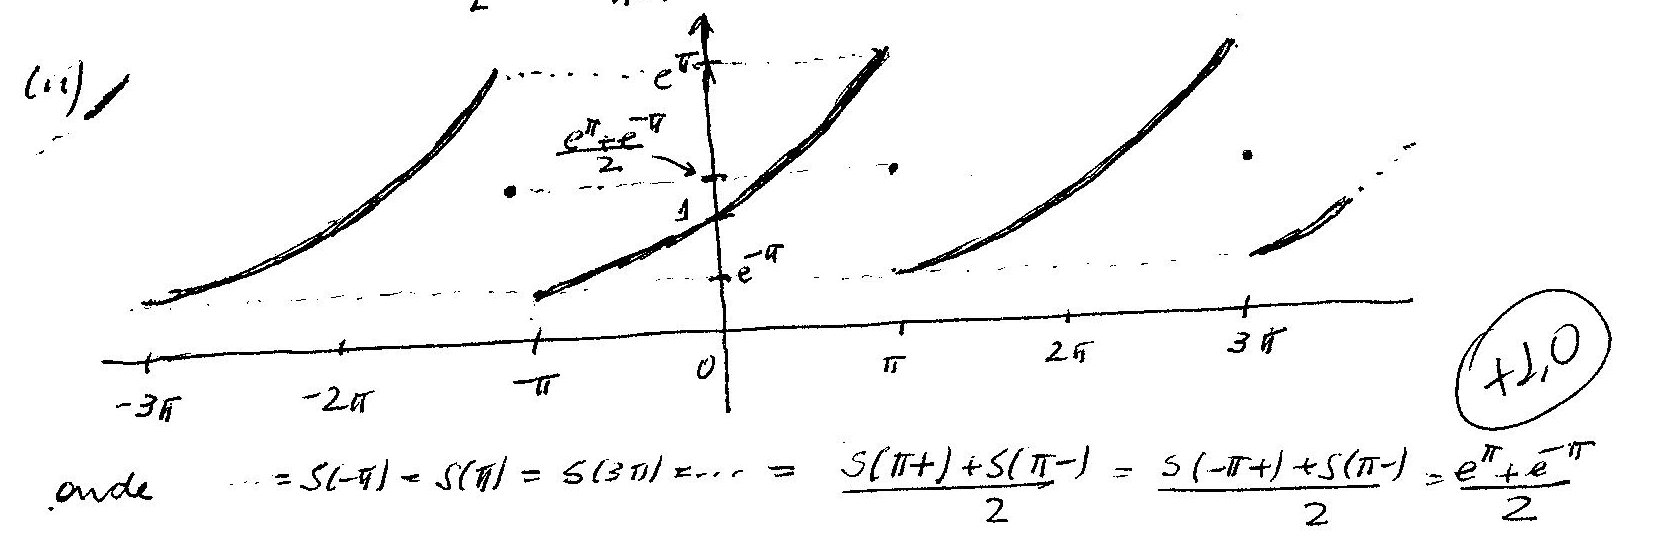
\includegraphics[width=0.8\textwidth]{lista1_fig_p1.jpg}
      \end{center}
    \end{solution}

    \part Use a série de Fourier para mostrar que
    \begin{align*}
      \sum_{n = 1}^\infty \frac{1}{n^2 + 1} &= \frac{\pi}{2} \coth\left( \pi \right) - \frac{1}{2}.
    \end{align*}
    \begin{solution}
      Tomando $x = \pi$ temos que
      \begin{align*}
        \frac{\exp(\pi) + \exp(-\pi)}{2} &= \cosh\left( \pi \right) \\
        &= \frac{2 \sinh(\pi)}{\pi} \left[ \frac{1}{2} + \sum_{n = 1}^\infty \frac{(-1)^n}{1 + n^2} \left( (-1)^n - n \cdot 0 \right) \right]
      \end{align*}
      e portanto
      \begin{align*}
        \sum_{n = 1}^\infty \frac{1}{1 + n^2} &= \frac{\pi}{2} \coth(\pi) - \frac{1}{2}.
      \end{align*}
    \end{solution}
  \end{parts}

  \question[T1 de 2012] Encontre a série de Fourier em senos no intervalo $[0,\pi]$ da função $f(x) = x \sin\left( 2 x \right)$, representada abaixo, e faça um gráfico da função representada por essa série para $x \in \mathbb{R}$.
  \begin{center}
    \begin{tikzpicture}[scale=.5]
      \draw[->] (-7,0) -- (7,0) node[below right]{$x$};
      \foreach \x in {1,...,6}{
      \node[below] at (\x,0) {$\x$};
      \node[below] at (-\x,0) {$-\x$};
      }
      \draw[->] (0,-6) -- (0,4.5) node[above right]{$x \sin\left( 2 x \right)$};
      \foreach \x in {1,...,4}{
      \node[left] at (0,\x) {$\x$};
      \node[left] at (0,-\x) {$-\x$};
      }
      \node[left] at (0,-5) {$-5$};
      \node[left] at (0,-6) {$-6$};

      \draw plot[domain=-6.5:6.5, samples=100] (\x, {\x * sin(2 * \x r)});
    \end{tikzpicture}
  \end{center}
  \begin{solution}
    A série de Foueier em senos é
    \begin{align*}
      f(x) &= \sum_{n = 1}^\infty b_n \sin\left( n x \right),
    \end{align*}
    onde
    \begin{align*}
      b_n &= \frac{2}{\pi} \int_0^\pi f(x) \sin\left( n x \right) \id{x}.
    \end{align*}

    Portanto,
    \begin{align*}
      b_n &= \frac{2}{\pi} \int_0^\pi x \sin\left( 2 x \right) \sin\left( n x \right) \id{x} \\
      &= \frac{2}{\pi} \int_0^\pi x \frac{1}{2} \left[ \cos\left( 2 x - n x \right) - \cos\left( 2 x + 2 n \right) \right] \id{x} \\
      &= \frac{1}{\pi} \underbrace{\int_0^\pi x \cos\left( \left( n - 2 \right) x \right) \id{x}}_{\bigstar} - \frac{1}{\pi} \underbrace{\int_0^\pi x \cos\left( \left( n + 2 \right) x \right) \id{x}}_{\bigstar\bigstar} \\
      \bigstar &= \begin{cases}
        \left[ (-1)^{n - 2} - 1 \right] \left( n - 2 \right)^{-2}, n \neq 2, \\
        \int_0^\pi x \cos\left( 0 x \right) \id{x} = \pi^2 / 2, n = 2,
      \end{cases} \\
      \bigstar\bigstar &= \underbrace{\left. x \frac{\sin\left( \left( n + 2 \right) x \right)}{n + 2} \right|_0^\pi}_{=0} - \frac{1}{n + 2} \int_0^\pi \sin\left( \left( n + 2 \right) x \right) \id{x} \\
      &= \left. \frac{1}{\left( n + 2 \right)^2} \cos\left( \left( n + 2 \right) x \right) \right|_0^\pi \\
      &= \frac{\left[ \left( -1 \right)^{n + 2} - 1 \right]}{\left( n + 2 \right)^2},
    \end{align*}

    Para $n \neq 2$, temos
    \begin{align*}
      b_n &= \frac{1}{\pi} \left[ \frac{\left[ (-1)^n - 1 \right]}{\left( n - 2 \right)^2} - \frac{\left[ \left( -1 \right)^n - 1 \right]}{\left( n + 2 \right)^2} \right] \\
      &= \frac{1}{\pi} \frac{\left[ \left( -1 \right)^n - 1 \right]}{\left( n^2 - 4 \right)^2} \left[ \left( n + 2 \right)^2 - \left( n - 2 \right)^2 \right] \\
      &= \frac{8 n}{\pi} \frac{\left[ \left( -1 \right)^n - 1 \right]}{\left( n^2 - 4 \right)^2}.
    \end{align*}
    E para $n = 2$, temos
    \begin{align*}
      b_2 &= \frac{1}{\pi} \left[ \frac{\pi^2}{2} - \frac{\left[ \left( -1 \right)^2 - 1 \right]}{\left( 2 + 2 \right)^2} \right] \\
      &= \frac{\pi}{2}.
    \end{align*}

    Por fim,
    \begin{align*}
      f(x) &= \frac{\pi}{2} \sin\left( 2 x \right) + \sum_{n = 1, n \neq 2}^\infty \frac{8 n}{\pi} \frac{\left[ (-1)^n - 1 \right]}{\left( n^2 - 4 \right)^2} \sin\left( n x \right) \\
      &= \frac{\pi}{2} \sin\left( 2 x \right) + \sum_{n = 1, 3, 5, \ldots}^\infty \frac{8 n}{\pi} \frac{\left[ (-1)^n - 1 \right]}{\left( n^2 - 4 \right)^2} \sin\left( n x \right) \\
      &= \frac{\pi}{2} \sin(2 x) - \frac{16}{\pi} \sum_{k = 0}^\infty \frac{\left( 2 k + 1 \right) \sin\left( \left( 2k + 1 \right) x \right)}{\left[ \left( 2 k + 1 \right)^2 - 4 \right]^2}.
    \end{align*}
    \begin{center}
      \begin{tikzpicture}[scale=.8]
        \draw[->] (-7,0) -- (7,0) node[below right]{$x$};
        \foreach \x in {1,...,6}{
        \node[below] at (\x,0) {$\x$};
        \node[below] at (-\x,0) {$-\x$};
        }
        \draw[->] (0,-6) -- (0,4.5) node[above right]{$x \sin\left( 2 x \right)$};
        \foreach \x in {1,...,4}{
        \node[left] at (0,\x) {$\x$};
        \node[left] at (0,-\x) {$-\x$};
        }
        \node[left] at (0,-5) {$-5$};
        \node[left] at (0,-6) {$-6$};

        \draw plot[domain=0:3.14] (\x, {\x * sin(2 * \x r)});
        \draw[xshift=3.14cm] plot[domain=0:3.14] (\x, {- (3.14 - \x) * sin(2 * (3.14 - \x) r)});
        \draw[xshift=-3.14cm] plot[domain=0:3.14] (\x, {- (3.14 - \x) * sin(2 * (3.14 - \x) r)});
        \draw[xshift=-6.28cm] plot[domain=0:3.14] (\x, {\x * sin(2 * \x r)});
      \end{tikzpicture}
    \end{center}
  \end{solution}

  \question[P1 de 2012] Considere a função $f(x) = x + x^2$. A série de Fourier
  no intervalo $[-\pi,\pi]$ de $f(x)$ é dada por
  \begin{dmath*}
    \frac{\pi^2}{3} + \sum_{n = 1}^{\infty} \left[ \frac{4}{n^2} (-1)^n \cos(n
    x) - \frac{2}{n} (-1)^n \sin(n x) \right].
  \end{dmath*}
  \begin{parts}
    \part Use esse resultado para calcular $\sum_{n = 1}^{\infty} 1 / n^2$.
    \begin{solution}
      Tomando $x = \pi$, temos, pela série de Fourier, que
      \begin{dmath*}
        f(\pi) = \frac{\pi^2}{3} + \sum_{n = 1}^{\infty} \left[ \frac{4}{n^2}
        (-1)^n \cos(n \pi) - \frac{2}{n} (-1)^n \sin(n \pi) \right]
        = \frac{\pi^2}{3} + \sum_{n = 1}^{\infty} \left[ \frac{4}{n^2}
        (-1)^n (-1)^n - \frac{2}{n} (-1)^n 0 \right]
        = \frac{\pi^2}{3} + \sum_{n = 1}^{\infty} \frac{4}{n^2}
        (-1)^n (-1)^n
        = \frac{\pi^2}{3} + \sum_{n = 1}^{\infty} \frac{4}{n^2}
        = \frac{1}{2} \left[ f(\pi + 0) + f(\pi - 0) \right]
        = \frac{1}{2} \left[ f(-\pi + 0) + f(\pi - 0) \right]
        = \frac{1}{2} \left[ \pi + \pi^2 + (-\pi + \pi^2) \right]
        = \pi^2.
      \end{dmath*}
      Logo,
      \begin{dmath*}
        \sum_{n = 1}^{\infty} \frac{4}{n^2} = \pi^2 - \frac{\pi^2}{3}
        = \frac{2 \pi^2}{3}.
      \end{dmath*}
      Portanto, $\sum_{n = 1}^{\infty} 1 / n^2 = \pi^2 / 6$.
    \end{solution}

    \part Faça um esboço, para $x \in \mathbb{R}$, do gráfico das funções
    repreentadas pelas séries nos casos: da série acima, da série de Fourier em
    cossenos no intervalo $[0,\pi]$ de $f(x)$ e da série de Fourier em senos no
    intervalo $[-\pi,0]$ de $f(x)$.
    \begin{solution}
      Esboço de $f(x)$:
      \begin{center}
        \begin{tikzpicture}
          \draw[->] (-2.2,0) -- (2.2,0) node[below right] {$x$};
          \draw[->] (0,-1) -- (0,7) node[above right] {$f(x)$};

          \draw[blue,domain=-2:2,samples=100] plot (\x, \x + \x * \x);
          
          \foreach \x in {-2,-1,...,2} {
            \draw (\x,0) node[below] {$\x \pi$};
          }
        \end{tikzpicture}
      \end{center}

      Esboço da série do item anterior:
      \begin{center}
        \begin{tikzpicture}
          \draw[->] (-6.2,0) -- (6.2,0) node[below right] {$x$};
          \draw[->] (0,-1) -- (0,7) node[above right] {$f(x)$};

          \foreach \s in {-4,0,4} {
            \draw[blue,domain=-2:2,samples=100] plot (\x + \s, \x + \x * \x);
          }

          \foreach \x in {-6,-5,...,6} {
            \draw (\x,0) node[below] {$\x \pi$};
          }
        \end{tikzpicture}
      \end{center}

      Esboço da série de Fourier em cossenos:
      \begin{center}
        \begin{tikzpicture}
          \draw[->] (-6.2,0) -- (6.2,0) node[below right] {$x$};
          \draw[->] (0,-1) -- (0,7) node[above right] {$f(x)$};

          \foreach \s in {-4,0,4} {
            \draw[blue,domain=0:2,samples=100] plot (\x + \s, \x + \x * \x);
            \draw[blue,domain=-2:0,samples=100] plot (\x + \s, -\x + \x * \x);
          }

          \foreach \x in {-6,-5,...,6} {
            \draw (\x,0) node[below] {$\x \pi$};
          }
        \end{tikzpicture}
      \end{center}

      Esboço da série de Fourier em senos:
      \begin{center}
        \begin{tikzpicture}
          \draw[->] (-6.2,0) -- (6.2,0) node[below right] {$x$};
          \draw[->] (0,-3) -- (0,3) node[above right] {$f(x)$};

          \foreach \s in {-4,0,4} {
            \draw[blue,domain=-2:0,samples=100] plot (\x + \s, \x + \x * \x);
            \draw[blue,domain=2:0,samples=100] plot (\x + \s, \x - \x * \x);
          }

          \foreach \x in {-6,-5,...,6} {
            \draw (\x,0) node[below] {$\x \pi$};
          }
        \end{tikzpicture}
      \end{center}
    \end{solution}
  \end{parts}
\end{questions}

\section{Lista de Integrais}
\begin{dmath}[label={ti:80}]
  \int \cos(a x) \sin(b x) \vi{x} = \frac{\cos\left( (a - b) x \right)}{4 (2 a -
  b)} - \frac{\cos\left( (a + b) x \right)}{2 (a + b)} \condition{$a \neq b$}
\end{dmath}

% \bibliographystyle{plain}
% \bibliography{bibliography}
\end{document}
